% The code is quite messy !!!

\documentclass[tikz,border=10pt]{standalone}

\begin{document}

    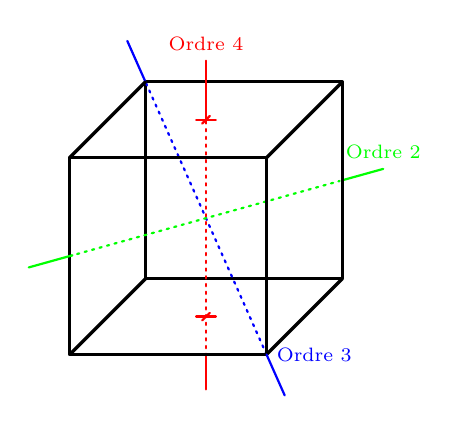
\begin{tikzpicture}[scale=2.5, line join=round, line cap=round]

        % Définir les sommets d'un cube
        \coordinate (A) at (0, 0, 0);
        \coordinate (B) at (1, 0, 0);
        \coordinate (C) at (1, 1, 0);
        \coordinate (D) at (0, 1, 0);
        \coordinate (E) at (0, 0, 1);
        \coordinate (F) at (1, 0, 1);
        \coordinate (G) at (1, 1, 1);
        \coordinate (H) at (0, 1, 1);
        
        \draw[green, thick] (1, 0.5, 0) -- (1.15, 0.5, -0.15) node[above, green] {\scriptsize Ordre 2};

        \draw[black, very thick] (A) -- (B) -- (C) -- (D) -- cycle; % Face de derriere
        
        % Axe d'ordre 4 (centre de deux faces opposées)
        \draw[red, thick, dotted] (0.5, -0.2, 0.5) -- (0.5, 1, 0.5);
        \draw[red, thick] (0.5, -0.37, 0.5) -- (0.5, -0.2, 0.5);
        \draw[red, thick] (0.5, 1, 0.5) -- (0.5, 1.3, 0.5) node[above, red] {\scriptsize Ordre 4};
        \draw[red, thick] (0.5, 0, 0.45) -- (0.5, 0, 0.55); % cross
        \draw[red, thick] (0.45, 0, 0.5) -- (0.55, 0, 0.5); % cross
        \draw[red, thick] (0.5, 1, 0.45) -- (0.5, 1, 0.55); % cross
        \draw[red, thick] (0.45, 1, 0.5) -- (0.55, 1, 0.5); % cross

        % Axe d'ordre 3 (grande diagonal)
        \draw[blue, thick, dotted] (1, 0, 1) -- (0, 1, 0);
        \draw[blue, thick] (0, 1, 0) -- (-0.15, 1.15, -0.15);

        % Axe d'ordre 2 (centre de deux aretes opposées)
        \draw[green, thick, dotted] (0, 0.5, 1) -- (0.99, 0.5, 0.01);
    

        % Tracer les arêtes du cube
        \draw[black, very thick] (E) -- (F) -- (G) -- (H) -- cycle; % Face supérieure

        \draw[green, thick] (0.01, 0.5, 0.99) -- (-0.15, 0.5, 1.15);

        \draw[black, very thick] (A) -- (E); % Arêtes verticales
        \draw[black, very thick] (B) -- (F);
        \draw[black, very thick] (C) -- (G);
        \draw[black, very thick] (D) -- (H);

        \draw[blue, thick] (1.15, -0.15, 1.15) -- (1, 0, 1) node[right, blue] {\scriptsize Ordre 3};
    \end{tikzpicture}

\end{document}